\newif\ifvimbug
\vimbugfalse

\ifvimbug
\begin{document}
\fi


\subsection{Quantisierung von Positionsdaten (4 Punkte)}
\subsubsection{2 Punkte}
Quantiesierung für b=2. Erster Pfeil Quantisierung und zweiter Pfeil Dekomprimierung.\\
$\begin{pmatrix} 0\\1 \end{pmatrix} \rightarrow \begin{pmatrix} 2\\3 \end{pmatrix} \rightarrow \begin{pmatrix} 1/3\\1 \end{pmatrix}\\
\begin{pmatrix} -0.7\\-0.7 \end{pmatrix} \rightarrow \begin{pmatrix}0\\0 \end{pmatrix} \rightarrow \begin{pmatrix} -1\\-1 \end{pmatrix}\\
\begin{pmatrix} 0.7\\0.7 \end{pmatrix} \rightarrow \begin{pmatrix} 3\\3 \end{pmatrix} \rightarrow \begin{pmatrix} 1\\1 \end{pmatrix}\\
\begin{pmatrix} -1\\0 \end{pmatrix} \rightarrow \begin{pmatrix} 0\\2 \end{pmatrix} \rightarrow \begin{pmatrix} -1\\1/3 \end{pmatrix}\\
\begin{pmatrix} 1\\0 \end{pmatrix} \rightarrow \begin{pmatrix} 3\\2 \end{pmatrix} \rightarrow \begin{pmatrix} 1\\1/3 \end{pmatrix}\\
\begin{pmatrix} -0.7\\0.7 \end{pmatrix} \rightarrow \begin{pmatrix} 0\\3 \end{pmatrix} \rightarrow \begin{pmatrix} -1\\1 \end{pmatrix}\\
\begin{pmatrix} 0.7\\-0.7 \end{pmatrix} \rightarrow \begin{pmatrix} 3\\0 \end{pmatrix} \rightarrow \begin{pmatrix} 1\\-1 \end{pmatrix}\\
\begin{pmatrix} 0\\0 \end{pmatrix} \rightarrow \begin{pmatrix} 2\\2 \end{pmatrix} \rightarrow \begin{pmatrix} 1/3\\1/3 \end{pmatrix}\\
\begin{pmatrix} 0\\-1 \end{pmatrix} \rightarrow \begin{pmatrix} 2\\0 \end{pmatrix} \rightarrow \begin{pmatrix} 1/3\\-1 \end{pmatrix}\\$

Quantiesierung für b=3.\\
$\begin{pmatrix} 0\\1 \end{pmatrix} \rightarrow \begin{pmatrix}4\\7 \end{pmatrix} \rightarrow \begin{pmatrix} 1/7\\1 \end{pmatrix}\\
\begin{pmatrix} -0.7\\-0.7 \end{pmatrix} \rightarrow \begin{pmatrix}1\\1 \end{pmatrix} \rightarrow \begin{pmatrix} -5/7\\-5/7 \end{pmatrix}\\
\begin{pmatrix} 0.7\\0.7 \end{pmatrix} \rightarrow \begin{pmatrix} 6\\6 \end{pmatrix} \rightarrow \begin{pmatrix}5/7 \\5/7\end{pmatrix}\\
\begin{pmatrix} -1\\0 \end{pmatrix} \rightarrow \begin{pmatrix} 0\\4 \end{pmatrix} \rightarrow \begin{pmatrix} -1\\1/7 \end{pmatrix}\\
\begin{pmatrix} 1\\0 \end{pmatrix} \rightarrow \begin{pmatrix} 7\\4 \end{pmatrix} \rightarrow \begin{pmatrix} 1\\1/7 \end{pmatrix}\\
\begin{pmatrix} -0.7\\0.7 \end{pmatrix} \rightarrow \begin{pmatrix} 1\\6 \end{pmatrix} \rightarrow \begin{pmatrix} -5/7\\5/7 \end{pmatrix}\\
\begin{pmatrix} 0.7\\-0.7 \end{pmatrix} \rightarrow \begin{pmatrix} 6\\1 \end{pmatrix} \rightarrow \begin{pmatrix} 5/7\\-5/7 \end{pmatrix}\\
\begin{pmatrix} 0\\0 \end{pmatrix} \rightarrow \begin{pmatrix} 4\\4\end{pmatrix} \rightarrow \begin{pmatrix} 1/7\\1/7 \end{pmatrix}\\
\begin{pmatrix} 0\\-1 \end{pmatrix} \rightarrow \begin{pmatrix} 4\\0 \end{pmatrix} \rightarrow \begin{pmatrix} 1/7\\-1 \end{pmatrix}\\$

<<<<<<< HEAD
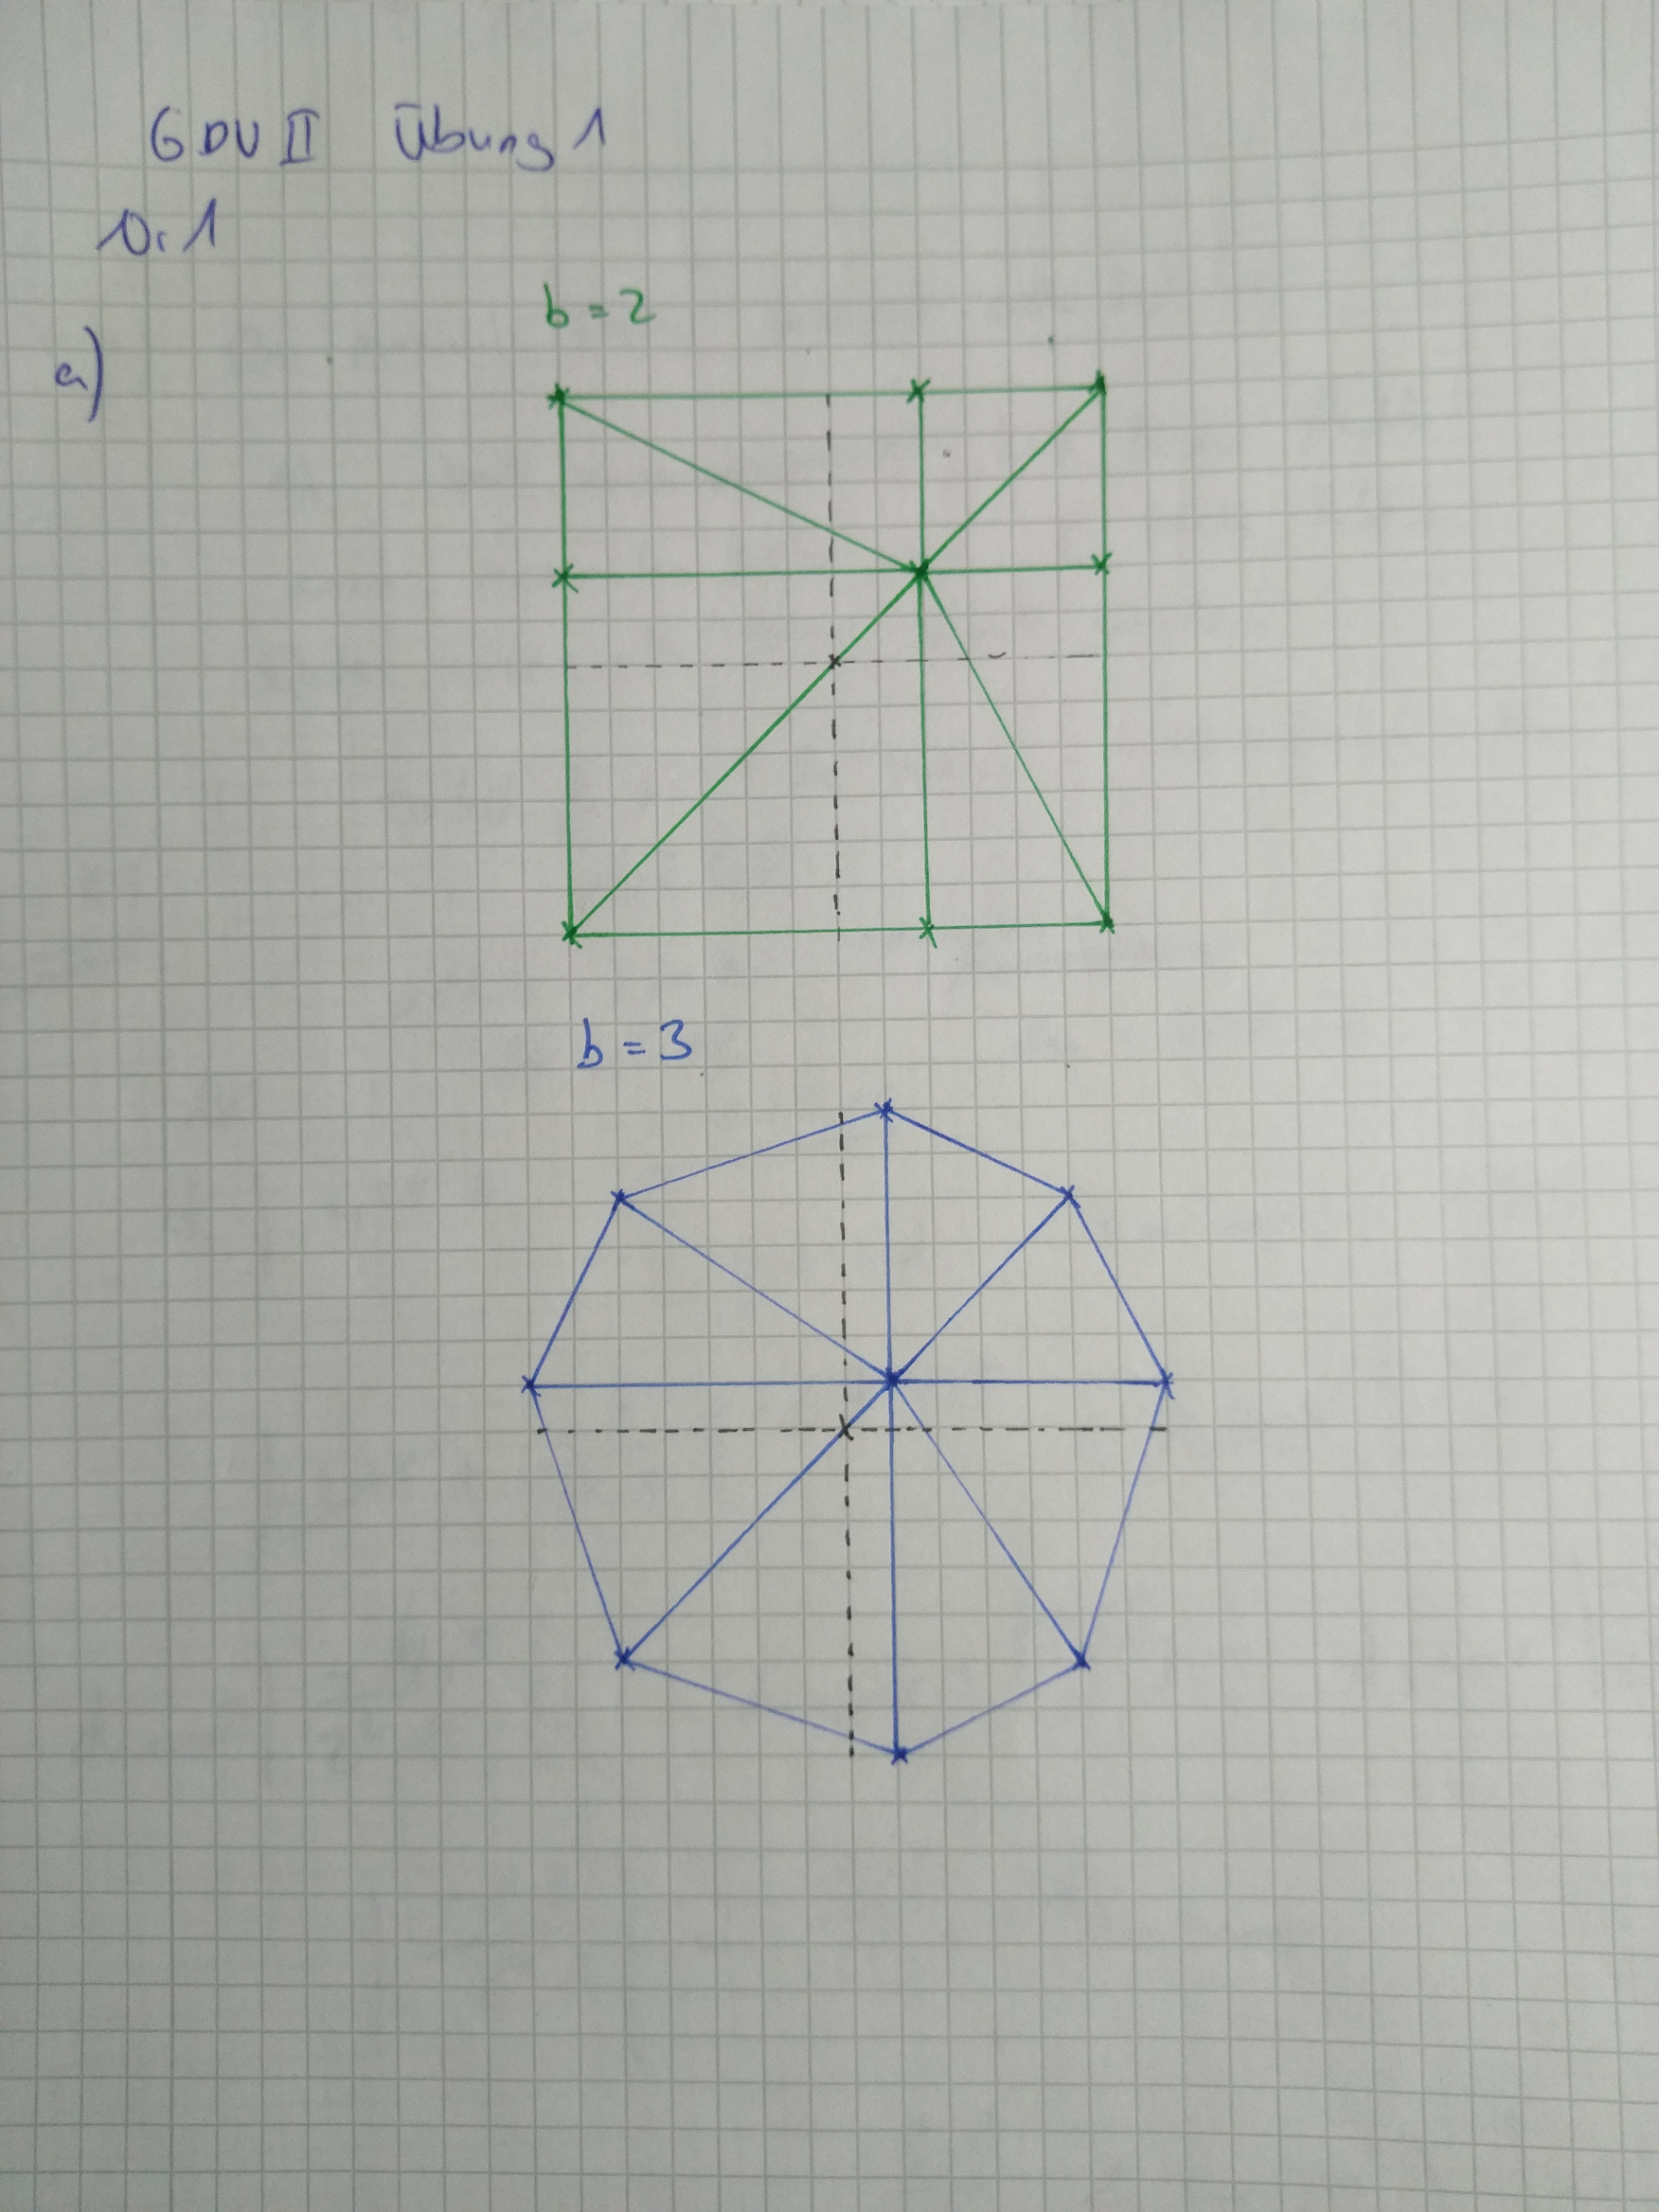
\includegraphics[scale=0.25]{1a_Zeichnung_J}

\subsubsection{2}
=======
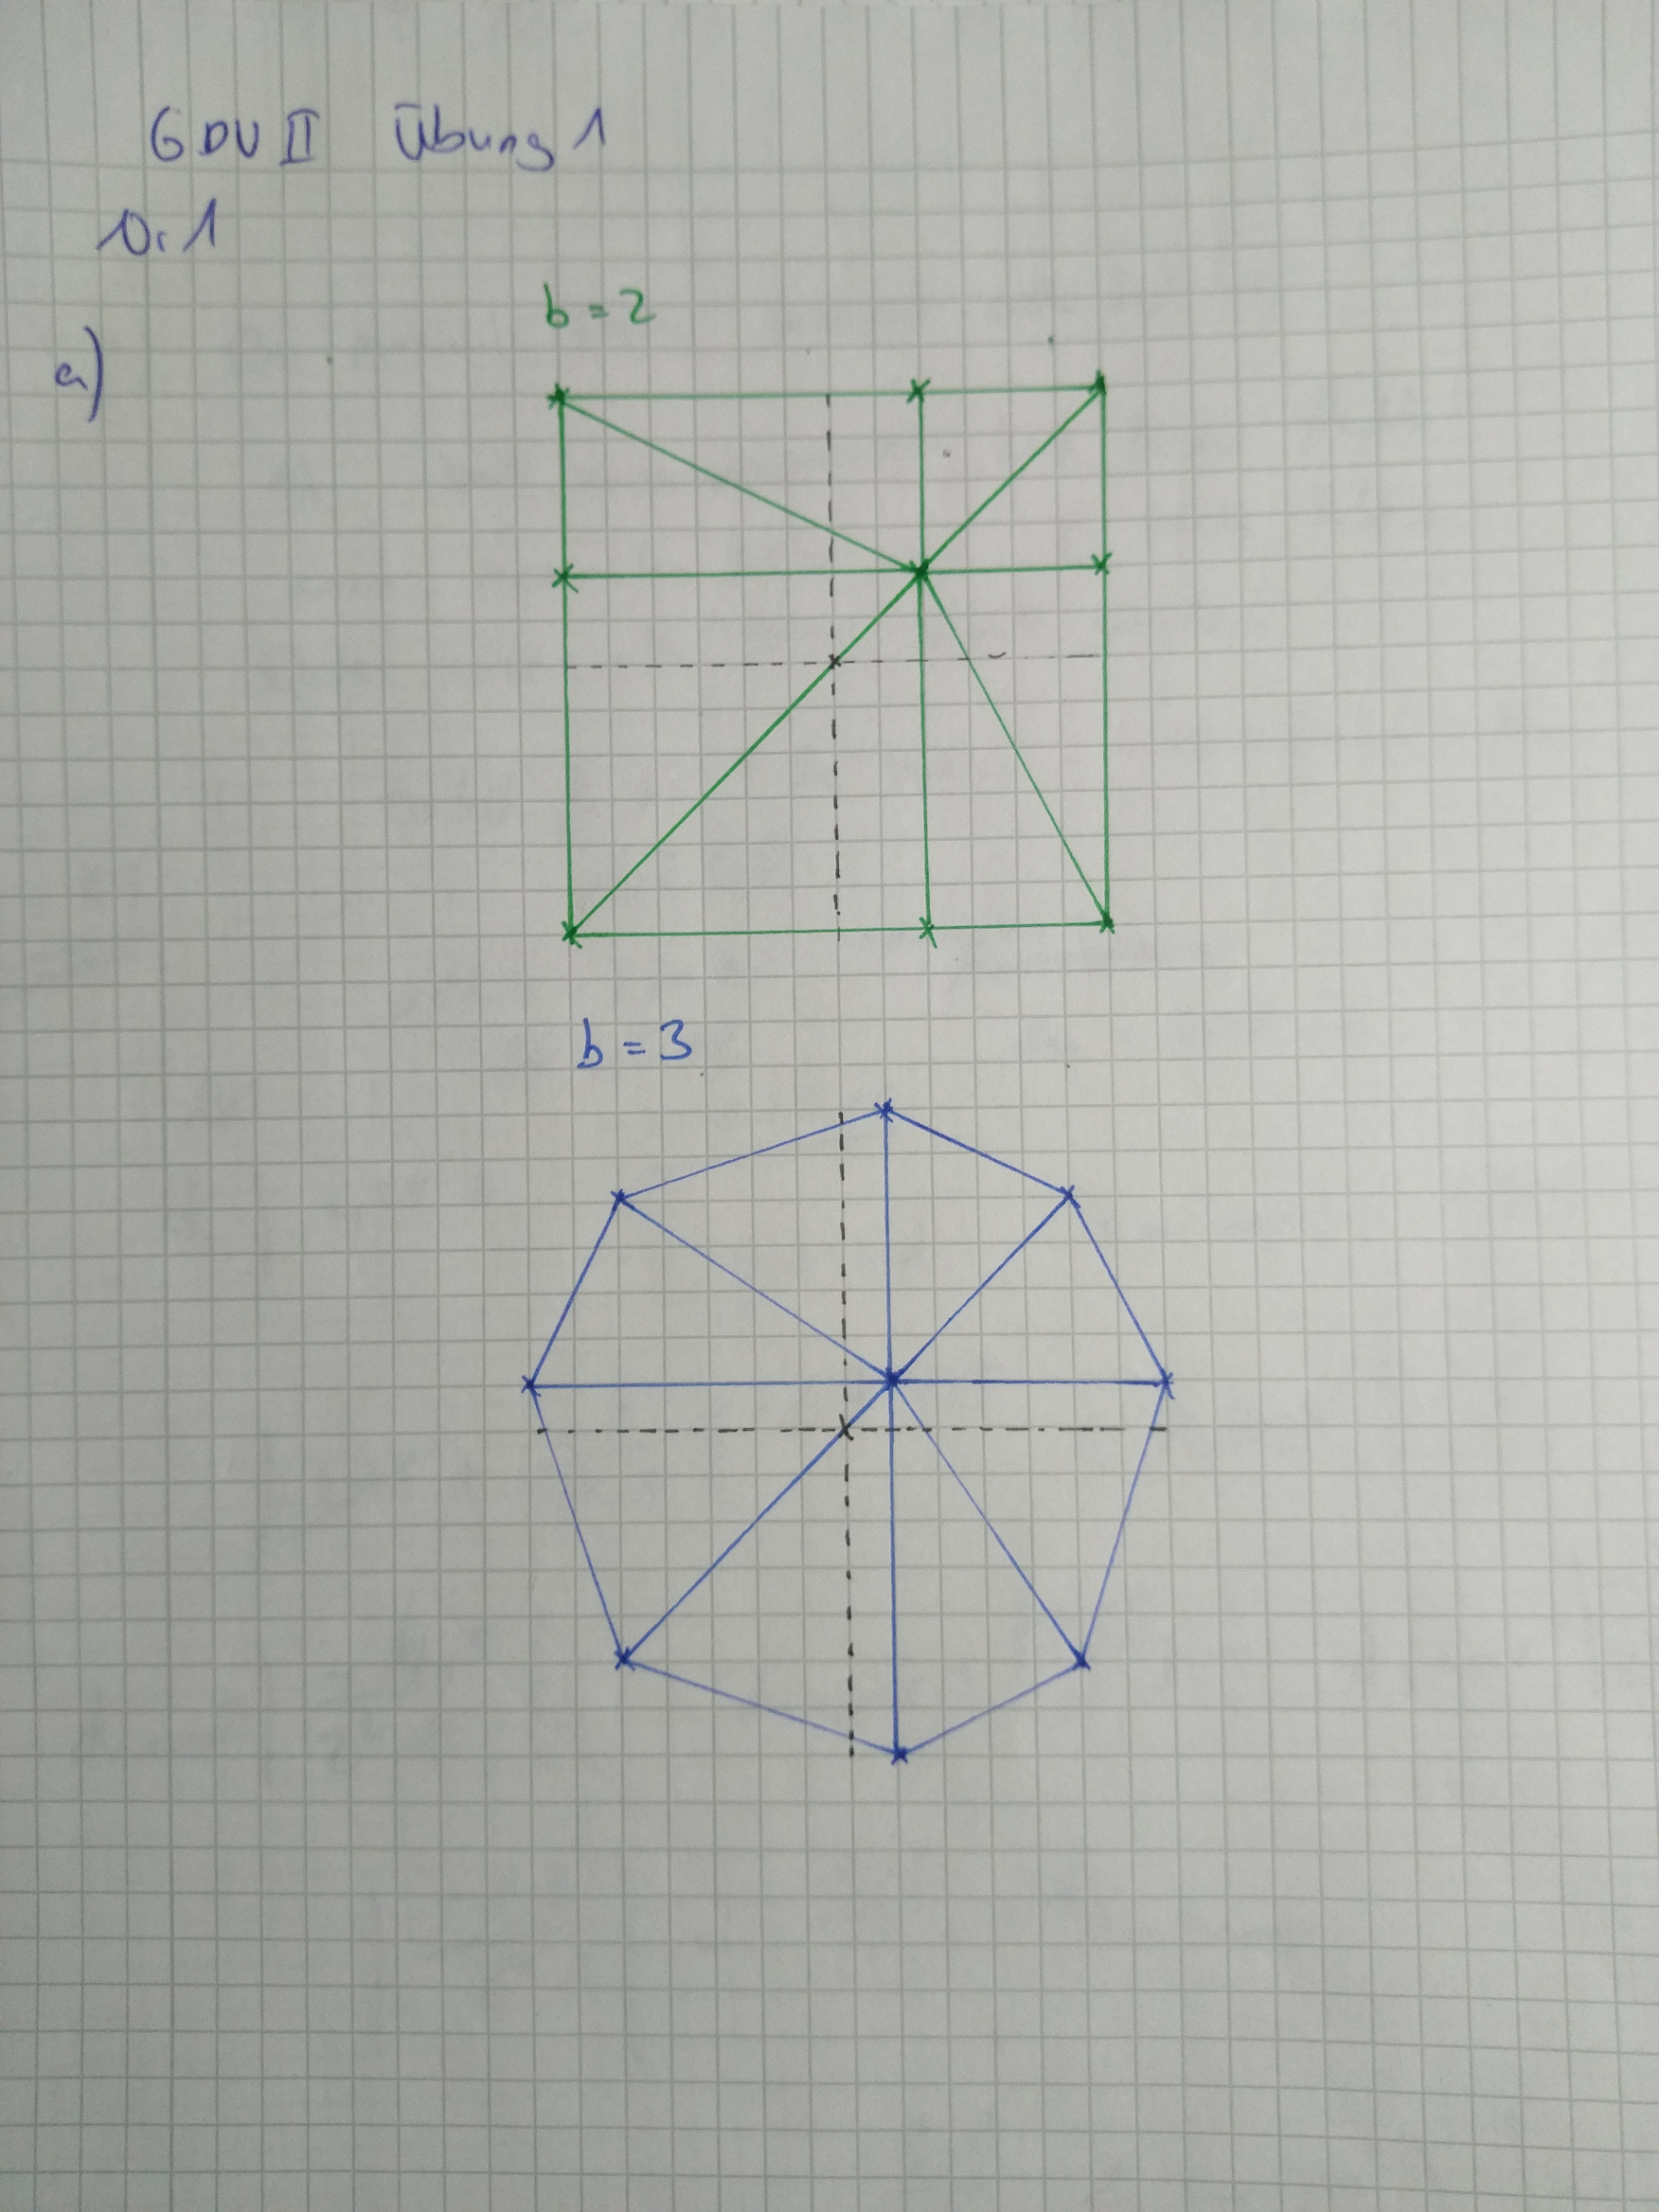
\includegraphics[height=9cm]{1a_Zeichnung_J.jpg}
>>>>>>> b9ce24dce1a570fcb0ae46d004a76d1d68135e22

\subsubsection{2 Punkte}

\subsubsection{1 Punkt}

